\documentclass{article}
\usepackage[utf8]{inputenc}

\title{PS7_Fillmore}
\author{benjaminpaynefillmore }
\date{March 2021}

\usepackage{graphicx}

\begin{document}
\graphicspath{ {./images/} }
\maketitle

\section{Main}
My imputations ultimately yield estimates of 0.062, 0.050,	0.062,	0.062 for the Listwise, Mean, Predicted, and MICE respectively. I would imagine this means I have done something incorrectly, as in my past experiences MICE has been significantly more accurate than any other form of imputation. 

For my project, I'm considering looking into scoring and assist figures for different Premier League teams, comparing performance in domestic and international competitions. I'll try to cluster by position and country of origin. Ideally, I'll be seeing if there is a distinct striker archetype that tends to have stronger performances in international play.


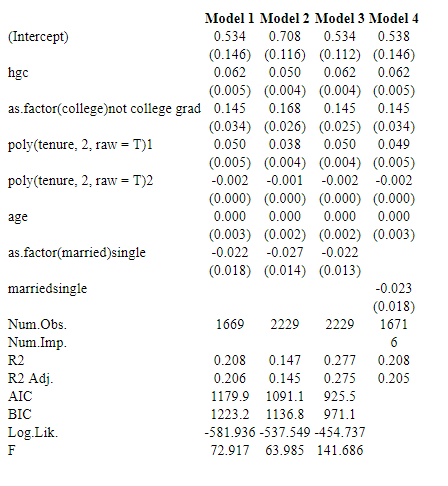
\includegraphics[width=\textwidth]{Images/modelsummary.png}


\end{document}
